%hello_world.tex
\documentclass[twocolumn]{article}
\usepackage{amsmath,amssymb}
\usepackage[amsmath,thref,thmmarks]{ntheorem}
%ntheorem宏包与amsmath有冲突,一起使用要加上amsmath选项
%使用定理环境的交叉引用,要加上thref选项;使用证明结束符,要加上thmmarks选项(?)
\usepackage{graphicx}
\usepackage{subfigure}
\usepackage{CJKutf8}
\usepackage{algorithm}
\usepackage{algorithmic}
\renewcommand\figurename{图}
\usepackage{geometry}
\usepackage{indentfirst}
\geometry{
left=3cm,
right=3cm,
top=3cm,
bottom=3cm}
\setlength{\parindent}{2em}
\setlength{\parskip}{0.5em}


\begin{CJK}{UTF8}{gbsn}
    \newtheorem{definition}{\hspace{2em}定义}
    \newtheorem{lemma}{\hspace{2em}引理}
    \newtheorem{theorem}{\hspace{2em}定理}
    \newtheorem{corollary}{\hspace{2em}推论}

    \theoremstyle{nonumberplain}%nonumberplain是不编号的定理环境
    \theoremsymbol{\ensuremath{\Box}}%设置定理结束符
    \newtheorem{proof}{\hspace{2em}证明}
\end{CJK}


% \setlength{}
\usepackage{cite}
% \usepackage{endnotes}
\title{
    \begin{CJK}{UTF8}{gbsn}
    组合问题中的可归约性
    \end{CJK}
    \thanks{This research was partially supported by National Science Foundation Grant CJ-474.}
    % \thanks{这项研究得到了美国国家科学基金会CJ-474的部分支持。}
}
\author{
    % \alignauthor
    \begin{CJK}{UTF8}{gbsn}
    作者
    \end{CJK}
    Richard M. Karp\\
    \begin{CJK}{UTF8}{gbsn}
    加州大学伯克利分校
    \end{CJK}
    \\
    \begin{CJK}{UTF8}{gbsn}
    译者 李其迈
    \end{CJK}
    \\
    \begin{CJK}{UTF8}{gbsn}
    浙江大学
    \end{CJK}
}
\date{}
% 实验内容,理论分析,实验细节,实验结果
\begin{document}
\maketitle

\begin{CJK}{UTF8}{gbsn}
\begin{abstract}
无向图、有向图、整数、数列、有限集合的有限族、布尔表达式等可数集中元素的性质判定问题构成了计算问题中相当大的一部分。通过简单的编码将这些可数集映射到一个定义在有限字母表上的串集中,这些问题可以被转化为语言的判定问题,籍此我们可以讨论它们的计算复杂性。当一个解终止所需要的计算次数是它的输入长度的多项式或更低阶函数,则认为这个解对应的问题得到了满意的解决。本文展示了许多经典的转化、匹配、装箱、路由、分配问题都是等价的,即它们要么全都是多项式时间可解问题,要么全都不是。
\end{abstract}

\section{引言}

    目前已知的所有用来计算图的色数,判定汉密尔顿回路存在性或者解0-1整数规划的方法的计算复杂度,在最坏的情况下,都随着其输入长度的指数函数。在本文中我们给出了一些定理,它们强烈的暗示这些问题永远都不会得到有效解决,但也只是暗示而已。

    我们对于多项式算法的存在性具有特别的兴趣。我们展示了一部分著名的组合问题,包括上文中提到的那些,它们是等价的,即任何一个问题存在多项式时间算法都可推出其它问题存在多项式时间算法。我们也证明了,如果这些问题存在多项式时间算法,一个出乎意料大的问题集合内的问题(简单的讲,所有通过回溯算法在多项式深度内可解的问题)都存在多项式时间算法。

    接下来是对本文内容的简短总结。明确的讲,我们所做的工作都是围绕着单带图灵机的语言判定问题来进行的,但是对于其它的抽象计算模型也有同样的理论。将所有0、1有限串组成的集合记为$\Sigma^*$。$\Sigma^*$的子集称为{\bf语言}。$\mathcal{P}$代表所有单带确定性图灵机上多项式时间内可判定的语言组成的集合。$\mathcal{NP}$代表所有单带非确定性图灵机上多项式时间内可判定的语言组成的集合。$\Pi$代表所有$\Sigma^*\to\Sigma^*$的单带确定性图灵机上多项式时间内可计算的函数。$L$和$M$各代表一个语言。如果存在一个函数$f\in\Pi$,使得($f(x)\in M)\Leftrightarrow(x\in L)$,则称$L${\bf 可归约到}$M$,记为$L\propto M$。如果$M\in\mathcal{P}$且$L\propto M$,则$L\in\mathcal{P}$。如果$L\propto M$且$M\propto L$则称$L$和$M$等价。如果$L\in\mathcal{NP}$且$\mathcal{NP}$中所有的语言都可以规约到$L$,则称$L$是({\bf多项式}){\bf完全}的。要么所有的完全语言都属于$\mathcal{P}$,要么都不是。当且仅当$\mathcal{P} = \mathcal{NP}$时,所有的完全语言都属于$\mathcal{P}$。

    本文的主要贡献是证明了一大批数学规划、图论、组合数学、计算逻辑学和开关理论中的经典计算问题,当他们转化为语言判定问题后,是完全的(因此也是等价的)。

    本文受到了Stephen Cook(1971)工作的启发,并且建立在他论文中介绍的一个重要定理之上。笔者同时也对 Eugene Lawler 和 Robert Tarjan 的潜在贡献表达感谢。

\section{$\mathcal{P}$类语言}
    无向图、有向图、整数、数列、有限集合的有限族、布尔表达式等可数集中元素的性质判定问题构成了计算问题中相当大的一部分。当且仅当存在一个算法,算法的运行时间被限定在输入长度的多项式或更低级别,这些问题被视为容易解决的。这个论断是合理且实用的,最早被 Jack Edmonds(1965) 提出,现在已经被广泛接受。这一节,我们将要介绍并且考察这一类多项式时间可解的问题。

    我们首先给出一个极度一般化的定义,定义出计算从可数定义域$D$到可数值域$R$的函数的确定性算法。

    对于任意有限字母表$A$,记$A$中元素构成的有限串所组成的集合为$A^*$;对于$x\in A^*$,记$x$的长度为$len(x)$。

    {\bf确定性算法}$\mathcal{A}\triangleq(D,R,\Delta,E,\tau)$,其中:
    \begin{itemize}
    \item $D$({\bf定义域})是一个可数集
    \item $R$({\bf值域})是一个可数集
    \item $\Delta$是字母表,且$\Delta^*\cap R=\Phi$
    \item E是{\bf编码函数} $E:D\rightarrow\Delta^*$
    \item $\tau$是一个{\bf转移函数 }$\tau:\Delta^*\rightarrow\Delta^*\cup R$
    \end{itemize}

    $\mathcal{A}$在输入$x\in D$上的{\bf计算}是一个唯一的串的序列$y1,y2,...$,且满足$y_1=E(x),y_{i+1}=\tau(y_i)$对于所有$i$,还要满足如果序列是有限的且结束于$y_k$,那么$y_k\in R$。任何计算过程中出现的串都被称为{\bf瞬时描述}。如果计算$\mathcal{A}$在输入x上的计算是有限的,且计算的长度为$t(x)$,那么$t(x)$被称为$\mathcal{A}$在$x$上的{\bf运行时间}。如果$\mathcal{A}$所有的计算都是有限的,则$\mathcal{A}$被称为{\bf停止的}。对于一个停止的算法$\mathcal{A}$,如果函数$f_\mathcal{A}:D\rightarrow R$对所有的$x$,$f_\mathcal{A}(x)$是$\mathcal{A}$在$x$上的计算的最后一个元素,则称$f_\mathcal{A}$是$\mathcal{A}$所计算的函数。

    如果$R=\{ACCEPT,REJECT\}$,那么$\mathcal{A}$被称为一个{\bf判定算法}。定义域$D=\Sigma^*$的判定算法被称为{\bf 串判定算法}。一个串判定算法$\mathcal{A}${\bf所判定的语言}为$\{x\in\Sigma^*|f_\mathcal{A}(x)=ACCEPT\}$。如果$D=R=\Sigma^*$,则$\mathcal{A}$被称为{\bf 串映射算法}。对于一个定义域为$D=\Sigma^*$停止的算法$\mathcal{A}$,如果存在一个多项式函数$p(\cdot)$使得对任意$x\in\Sigma^*$,有$t(x)\le p(len(x))$,则称$\mathcal{A}${\bf运行在多项式时间内}。

    在任何使用语境下讨论算法,我们都必须明确确定性算法的概念。各种不同类型的著名串判定算法(马尔科夫算法、单带图灵机、多带多头图灵机、随机存取机等)都限制函数$E$和$\tau$为简单明确的类型。对于这些概念,这里都使用标准的定义[Hopcroft \& Ullman(1969)],不在进行赘述。今天人们已经发现这些类型的算法在他们判定语言的能力上是等价的;对于任意一个类型的算法,它所能判定的语言组成的集合都是递归语言集。这种不受计算模型定义影响的不变性暗示着递归是可判定性概念的正确定义方法。

    可以被串判定算法在多项式时间内判定的语言组成的集合同样不随算法类型而改变。举个例子,任何一个可以在$p(\cdot)$时间内被多带图灵机判定的语言,都可以被单带图灵机在$p^2(\cdot)$时间内判定。因此单带图灵机多项式时间可判定的语言和更强大的多带图灵机在多项式时间内可判定的语言是一样的。类似的,随机读取机也有同样的性质。
    \begin{definition}
        $\mathcal{P}$ 是可以被单带图灵机在多项式时间内判定的语言的集合。
    \end{definition}
    \begin{definition}
        $\Pi$ 是所有可以被单带图灵机在多项式时间内计算的$\Sigma^*\to\Sigma^*$的函数的集合。
    \end{definition}

    读者可以把$\mathcal{P}$理解为可以被(内存无限的)数码计算机在多项式时间内判定的语言,把$\Pi$理解为可以被这种计算机在多项式时间内完成的串映射。这种理解是正确的。

    {\bf注意到},如果$f:\Sigma^*\to\Sigma^*$属于$\Pi$,那么就有一个多项式函数$p(\cdot)$,使得$len(f(x))\le p(len(x))$。

    我们接下来介绍规约的概念。规约的概念是本文的重中之重。
    \begin{definition}
        对于语言$L$和$M$,如果存在一个函数$f\in\Pi$,使得$f(x)\in M \Leftrightarrow x\in L$,则称$L${\bf 可归约到}$M$,记为$L\propto M$。
    \end{definition}

    \begin{lemma}
        如果$L\propto M$且$M \in \mathcal{P}$,那么$L\propto\mathcal{P}$。
    \end{lemma}
    \begin{proof}
        下面给出一个多项式时间算法来判定$x$是否属于$L$:计算$f(x)$,之后在多项式时间内判断是否有$f(x)\in M$。
    \end{proof}

    除了$\Sigma^*$,我们也对判定其它可数集的子集的难度感兴趣。给定集合$D$,就有一个很自然的一对一的编码函数$e:D\to\Sigma^*$。举个例子,我们可以把正整数编码成0-1串,把一维数组编码成整数列表,把矩阵编码成一维数组的列表,等等。而把列表编码成有限字符集的串,把有限字符集的串编码成0-1串,都是有标准方法可以遵循的。给定一个编码$e:D\to\Sigma^*$和集合$T\subseteq D$,如果$e(T)\in\mathcal{P}$,我们说集合$T${\bf多项式时间可判定}。同样的,给定$T\subseteq D$和$U\subseteq D'$以及编码函数$e:D\to\Sigma^*$和$e':D'\to\Sigma^*$,如果$e(T)\propto e'(U)$,则称$T\propto U$。

    一个可数集存在多种自然编码方式是可能的。举个例子,一个图可以被表示成邻接矩阵,关联矩阵,或者是边对应的顶点对的无序列表。对于以上任何一种表示方式,不同的格式,标点也会形成不同的编码。幸运的是,大多数时候对同一个问题的两种合理的编码$e_0,e_1$都是明显等价的,即$e_0(S)\in\mathcal{P}\Leftrightarrow e_1(S)\in\mathcal{P}$。一个重要的例外是正整数编码应该以二进制的形式编码,而不是一进制。注意到多项式时间内可判定性的不变性,我们都会在问题的原始集合内展开讨论,不再指定一个到$\Sigma^*$的编码。

    我们以一个多项式时间内可解问题的列表作为本节的结束。下一节,我们将考察一部分目前还没有多项式解法的问题的紧密关系。附录I有我们在这里使用的符号表。

    每一个问题会给出问题空间中元素的一般化表示(输入),以及导致输入被“接受”的性质。

    \begin{itemize}
    \item {\bf每一个clause最多有两个literal的可满足性问题}[Cook(1971)]\\
    输入:语句(Clause) $C_1,C_1,\cdots,C_p$,每一个都包含最多两个文字(literal)。\\
    性质:这些给定的语句 的合取是可满足的。也就是说存在集合$S\subseteq\{x_1,x_2,\cdots,x_n,\bar{x_1},\bar{x_2},\cdots,\bar{x_n}\}$,使得 \\
    a) S 不包含互补的文字。\\
    b) $S\cap C_k \neq \Phi, k = 1,2,\cdots,p$。

    \item {\bf最小生成树}[Kruskal(1956)]\\
    输入:$G, w, W$\\
    性质: 存在一个权值小于等于$W$最小生成树

    \item {\bf最短路问题}[Dijkstra(1959)]\\
    输入:$G, w, W, s, t$\\
    性质: 存在一个$s$到$t$的权值小于等于$W$的路径

    \item {\bf最小割}[Edmonds \& Karp(1972)]\\
    输入:$G, w, W, s, t$\\
    性质: 存在一个权值小于$W$的$s-t$割

    \item {\bf边覆盖}[Edmonds(1965)]\\
    输入:$G, k$\\
    性质: 存在一个集合$Y\subseteq A$,使得$|Y|\le k$且每个节点都与一个$Y$中的边临接。

    \item {\bf边删除}\\
    输入:$G, k$\\
    性质: 存在$k$个边组成的集合,删除这些边后,所有的环都不存在。

    \item {\bf偶匹配}[Hall(1948)]\\
    输入:$S\subseteq Z_p \times Z_p $\\
    性质: 输入中的有序对代表图的边。要求的性质为$S$代表一个二分图的边集。

    \item {\bf带有截止期限的排序}[Hall(1948)]\\
    输入:$(T_1,\cdots,T_n)\in Z^n, (D_1,\cdots,D_n)\in Z^n, k$\\
    性质: 一个人从0时刻开始进行工作$1,2,\cdots,n$,这些工作需要的工时为$T_i$,且各自的截止期限为$D_i$。在某些顺序下可以保证不超过$k$个工作错过截止期限。

    \item {\bf线性方程的有解性}[Hall(1948)]\\
    输入:$(c_{ij}), (a_i)$\\
    性质: 存在一个向量$(y_j)$,使得对所有$i$有$\sum_j c_{ij}y_j = a_i$
    \end{itemize}

\section{非确定性算法以及Cook定理}
    在本节中,我们陈述了Cook提出的一个重要定理。该定理表明,在$\mathcal{NP}$这一类相当大的语言都可以规约到一个特定的集合$S$。集合$S$对应问题是判定一个合取范式的布尔表达式是否可满足。
    记$\Sigma^*\times\Sigma^*$中所有可以在多项式时间内判定的子集组成的集合为$\mathcal{P}^{(2)}$。给定$L^{(2)}\in \mathcal{P}^{(2)}$以及一个多项式函数$p$,我们定义语言$L$如下:
    \begin{equation}\nonumber
        \begin{aligned}
            L=\{&x|\text{存在一个}y\text{使得}<x,y>\in L^{(2)} \\
                &\text{且}len(y)<p(len(x))\} \\
        \end{aligned}
    \end{equation}
    我们称$L$是根据p-bounded existential quantification从$L^{(2)}$中导出的语言。

    \begin{definition}
        根据polynomial-bounded existential quantification 从$\mathcal{P}^{(2)}$中的元素导出的语言组成的集合称为$\mathcal{NP}$。
    \end{definition}

    $\mathcal{NP}$中的语言有另外一个跟非确定性图灵机相关的刻画方式。一个{\bf非确定性判定算法}$\mathcal{A}\triangleq(D,\Delta,E,\tau)$,其中:
    \begin{itemize}
    \item $D$({\bf定义域})是一个可数集
    \item $\Delta$是字母表, \\
        且$\Delta^*\cap \{ACCEPT,REJECT\}=\Phi$
    \item E是{\bf编码函数} $E:D\rightarrow\Delta^*$
    \item $\tau$是一个{\bf转移关系} \\
        $\tau\subset\Delta^*\times(\Delta^*\cup \{ACCEPT,REJECT\})$
    \end{itemize}
    并且要求,对于所有$y_0 \in \Delta^*$,集合$\{<y_0,y>|<y_0,y>\in \tau\}$有少于$k_\mathcal{A}$个元素,其中$k_\mathcal{A}$是个常数。一个的$\mathcal{A}$在输入$x\in D$的{\bf计算}是一个序列$y_1,y_2,\cdots$,使得对$\forall i$有$y_1=E(x),<y_i,y_{i+1}\in\tau>$,并且,如果序列是有限的并且以$y_k$结尾,那么$y_k \in \{ACCEPT,REJECT\}$. 一个出现在某个计算中的串$y$被称为一个{\bf瞬时描述}。一个有限的且停止在$ACCEPT$上的计算被称为一个{\bf接受的计算}。对于输入$x$,如果存在一个接受的计算,则称$x$被{\bf接受}。如果$D=\Sigma^*$,那么我们称$\mathcal{A}$是一个{\bf非确定性串判定算法}。如果存在一个多项式函数$p(\cdot)$使得,对于所有$\mathcal{A}$接受的串$x$,都存在一个长度$\leq p(len(x))$的接受的计算,则称$\mathcal{A}${\bf运行在多项式时间内}。

    一个非确定性算法可以被视为是一个这样的过程。每当需要在两个计算方向中做选择,他就制造两个自己的复制品,然后两个复制品各自继续一个计算方向。像这样连续分裂可能导致复制品个数按指数级增长。有任何一个复制品接受了输入,则认为输入被这个算法接受。

    非确定性的单带图灵机、多带图灵机、随机读取机等通过把编码函数$E$和转移关系$\tau$限定在特别的形式,定义了各自的非确定性串识别算法。所有这些算法定义的多项式时间内可判定的语言集合是相同的。更确切的说,这个集合是$\mathcal{NP}$。

    \begin{theorem}
      $L\in \mathcal{NP}$当且仅当$L$被某个运行在多项式时间内的非确定性图灵机接受。
    \end{theorem}

    \begin{proof}
         

        $\Rightarrow$假设$L\in\mathcal{NP}$。那么,对于某个$L^{(2)}\in\mathcal{P}^{(2)}$以及某个多项式函数$p$,$L$是根据p-bounded existential quantification从$L^{(2)}$导出的语言。我们可以构造一个非确定机器。对于输入$x$,它首先猜测长度$\leq p(len(x))$的串\footnote{此处原文为$p(len(x))$,应是笔误}$y$,然后检测是否有$<x,y>\in L^{(2)}$。显然,这个机器在多项式时间内判定了$L$。

        $\Leftarrow$如果$L$被一个运行在多项式时间$p$内的非确定性图灵机$T$所接受。不失一般性的,我们假设对于任意瞬时描述$Z$,最多存在两个瞬时描述可以由$Z$转移到(也就是说,最多有两个可以选择的转移)。那么,对于一个给定的计算,$T$产生的瞬时描述序列可以被编码成一个0-1串,且$len(y)\leq p(len(x))$

        因此我们可以构造一个定义域为$\Sigma^*\times\Sigma^*$的确定性图灵机$T'$。这个图灵机在它的输入$<x,y>$上,模拟$T$在在输入$x$上,选择序列为$y$时的行为。显然,$T'$是运行在多项式时间内的,所以$L$是一个根据polynomial bounded existential quantification从一个被$T'$接受的串对集合中导出的。
    \end{proof}

    集合$\mathcal{NP}$非常庞大。不严格的讲,一个判定问题属于$\mathcal{NP}$当且仅当它可以被回溯搜索在多项式深度内解决。有很多重要的计算问题现在还无法证明属于$\mathcal{P}$,但是它们都明显属于$\mathcal{NP}$。比如着色问题————判断一个图中的节点被$k$种颜色着色后,是否能够使得相邻的节点都具有不同的颜色。一个非确定性的算法可以简单的猜一个颜色分配,然后在多项式时间内验证是否所有的相邻节点都有不同的颜色。

    考虑到$\mathcal{NP}$的范围如此之大,下面这个Cook提出的定理就非常有意义了。我们定义可满足性问题(简称SAT)如下:\\
    {\bf可满足性问题(SATISFIABILITY)}\\
    输入:语句(Clause) $C_1,C_2,\cdots,C_p$\\
    性质:给定语句的合取是可满足的;即存在集合$S\subseteq\{x_1,x_2,\cdots,x_n,\bar{x_1},\bar{x_2},\cdots,\bar{x_n}\}$同时满足:\\
    \indent a) S不存在互补的文字(literal)\\
    \indent b) $S\cap C_K\neg\Phi,k=1,2,\cdots,P$。

    \begin{theorem}[Cook]
        如果$L\in\mathcal{NP}$,那么$L\propto SAT$
    \end{theorem}

    Cook(1971)陈述该定理时,用的是一种并不能明确体现规约的记号,但是现在的这种陈述方式是建立在他的证明之上的。

    \begin{corollary}
        $P=\mathcal{NP} \Leftrightarrow SAT \in \mathcal{P}$
    \end{corollary}

    \begin{proof}
      如果$SAT\in\mathcal{P}$,那么对于所有的$L\in\mathcal{NP},L\in\mathcal{P}$,因为$L \propto SAT$。如果$SAT\not\in\mathcal{P}$,因为$SAT\in\mathcal{NP}$,那么$\mathcal{P}\neq\mathcal{NP}$。
    \end{proof}

    {\bf注意},如果$\mathcal{P}=\mathcal{NP}$,那么$\mathcal{NP}$关于补运算和polynomial-pounded existential quantification是封闭的。因此它关于polynomial-bounded universal quantification也是封闭的。接下来,polynomial-bounded analogue of Kleene's Arithmetic Hierarchy[Rogers(1967)]就变得平凡了,如果$\mathcal{P}=\mathcal{NP}$。

    定理2表明,如果存在一个多项式时间算法可以判定$SAT$问题,那么所有可以被多项式深度回溯搜索解决的问题都可以被多项式时间算法解决。这是对$SAT\not\in\mathcal{P}$的强烈暗示。

\section{完全问题}
    这篇论文的主要目标是找到一批和$SAT$问题有着相同地位的计算问题。这些问题可以被称为完全。
    \begin{definition}
        语言$L$被称为({\bf多项式}){\bf完全},当且仅当$L$同时满足:\\
        \indent a) $L\in\mathcal{NP}$\\
        \indent b) $SAT\propto L$\\
    \end{definition}

    \begin{theorem}
        要么所有的完全语言都属于$\mathcal{P}$,要么都不是。当且仅当$\mathcal{P}=\mathcal{NP}$时,前一种可能为真。
    \end{theorem}

    我们可以把完全的概念从定义在$\Sigma^*$上的语言扩展到定义在可数集上的问题。
    
    \begin{definition}
        $D$是一个可数集,$e$是一个“标准”的一对一编码函数$e:D\rightarrow\Sigma^*$且$T$是$D$的一个子集。那么$T$是{\bf完全}的,当且仅当$e(T)$是完全的\footnote{此处原文为$e(D)$,应是笔误}。
    \end{definition}

    \begin{lemma}
        用$D$和$D'$表示可数集,且有一对一编码函数$e$和$e'$。他们分别有子集$T\subset D$和$T'\subset D'$。如果存在函数$F:D\rightarrow D'$同时满足以下条件,则称$T\propto T'$。\\
        \indent a) $F(x)\in T' \Leftrightarrow x\in T$\\
        \indent b) 存在一个函数 $f\in\Pi$,使得 $f(x)=e'(F(e^{-1}(x)))$,只要$e'(F(e^{-1}(x)))$是有定义的。\\
    \end{lemma}

    本文的剩余部分主要进行了下面这个定理的证明。

    {\bf主要定理},以下列出的所有问题都是完全的。

    \begin{enumerate}
    \item {\bf可满足性问题(SATISFIABILITY)}\\
    注: 默认的,这个问题等价于判定一个析取范式是否是一个永真式。

    \item {\bf0-1整数规划问题\\(0-1 INTEGER PROGRAMMING)}\\
    输入:整数矩阵$C$和整数向量$d$\\
    性质:存在一个0-1向量$x$使得$Cx=d$

    \item {\bf分团问题(CLIQUE)}\\
    输入:图$G$,正整数$k$\\
    性质:存在$G$中$k$个互不相邻的节点组成的集合。

    \item {\bf(SET PACKING)}\\
    输入:一族集合$\{S_j\}$,正整数$\ell$\\
    性质:$\{S_j\}$包含$\ell$个互斥集合。

    \item {\bf顶点覆盖(NODE COVER)}\\
    输入:图$G'$,正整数$\ell$\\
    性质:存在集合$R\subset N'$,使得$|R|\leq\ell$且每一条边都与$R$中的某个顶点相邻。

    \item {\bf集合覆盖(SET COVERING)}\\
    输入:有限集合组成的有限族$\{S_j\}$,正整数$k$\\
    性质:存在一个子族$\{T_h\}\subset\{S_j\}$包含小于等于$k$个集合使得$\bigcup T_h=\bigcup S_j$。

    \item {\bf反馈顶点集(FEEDBACK NODE SET)}\\
    输入:有向图$H$,正整数$k$\\
    性质:存在一个集合$R\subset V$,使得$H$中的每个(有向)环包含一个$R$中的节点。

    \item {\bf反馈边集(FEEDBACK ARC SET)}\\
    输入:有向图$H$,正整数$k$\\
    性质:存在一个集合$S\subset E$,使得$H$中的每个(有向)环包含一个$S$中的边。

    \item {\bf有向汉密尔顿回路(DIRECTED HAMILTON CIRCUIT)}\\
    输入:有向图$H$\\
    性质:$H$存在一个有向环,经过图中每个节点恰好一次。

    \item {\bf无向汉密尔顿回路(UNDIRECTED HAMILTON CIRCUIT)}\\
    输入:图$G$\\
    性质:$G$存在一个环,经过图中每个节点恰好一次。

    \item {\bf3-可满足性问题\\(SATISFIABILITY WITH AT MOST 3 LITERALS PER CLAUSE)}\\
    输入:语句 $D_1,D_2,\cdots,D_r$,每个都最多包含3个文字(Literal)。\\
    性质:集合$\{D_1,D_2,\cdots,D_r\}$是可满足的

    \item {\bf色数(CHROMATIC NUMBER)}\\
    输入:图$G$,正整数$k$\\
    性质:存在一个函数$\Phi:N\rightarrow Z_k$,使得对任意相邻的顶点$u$和$v$,有$\Phi(u)\neq\Phi(v)$

    \item {\bf分团覆盖(CLIQUE COVER)}\\
    输入:图$G'$,正整数$\ell$\\
    性质:$N'$是$\ell$个或更少的团的并。

    \item {\bf精确覆盖(EXACT COVER)}\\
    输入:集合$\{u_i,i=1,2,\cdots,t\}$的子集组成的族${S_j}$\\
    性质:存在一个子族$\{T_h\}\subset\{S_j\}$,使得$T_h$两两互斥,且$\bigcup T_h=\bigcup S_j=\{u_i,i=1,2,\cdots,t\}$。

    \item {\bf碰集(HITTING SET)}\\
    输入:集合$\{s_j,j=1,2,\cdots,t\}$的子集组成的族${U_i}$\\
    性质:存在一个集合$W$,使得对于所有$i$,$|W\cap U_i|=1$

    \item {\bf斯坦纳树(STEINER TREE)}\\
    输入:图$G$,$R\subset N$,权重函数$w:A\rightarrow Z$,正整数$k$\\
    性质:G有一个权重小于等于$k$的子树,包含所有$R$中的节点

    \item {\bf三维匹配(3-DIMENSIONAL MATCHING)}\\
    输入:集合$U\subset T\times T\times T$,其中$T$是一个有限集\\
    性质:存在一个集合$W\subset U$,使得$|W|=|T|$,且$W$中任意两个元素在任意一个维度上的值都不相同。

    \item {\bf背包(KNAPSACK)}\\
    输入:$(a_1,a_2,\cdots,a_r,b)\in Z^{n+1}$(\\
    性质:$\sum a_j x_j=b$有0-1解

    \item {\bf工作排序(JOB SEQUENCING)}\\
    输入:“执行时间向量” $(T_1,\cdots,T_p)\in Z^p$\\
    \hphantom{输入:}“结束期限向量” $(D_1,\cdots,D_p)\in Z^p$\\
    \hphantom{输入:}“惩罚向量” $(P_1,\cdots,P_p)\in Z^p$\\
    \hphantom{输入:}正整数$k$\\
    性质:存在一个$\{1,2,\cdots,p\}$的排列$\Pi$使得:
    \begin{equation}\nonumber
        \begin{aligned}
            \sum_{j=1}^{p} [ \ {\tt if}\  T_{\Pi(1)}+\cdots+&T_{\Pi(j)} > D_{\Pi(j)} \\
                            & {\tt then} \  P_{\Pi(j)}\ {\tt else}\  0 \  ] \leq k
        \end{aligned}
    \end{equation}

    \item {\bf集合划分(PARTITION)}\\
    输入:$(c_1,c_2,\cdots,c_s)\in Z^s$\\
    性质:存在一个集合$I\subset\{1,2,\cdots,s\}$使得:
    $$\sum_{h\in I}c_h = \sum_{h\notin I}c_h$$

    \item {\bf最大割}\\
    输入:图$G$,权重函数$w:A\rightarrow Z$,正整数$W$\\
    性质:存在一个集合$S\subset N$,使得:
    $$\sum_{\substack{\{u,v\}\in A \\ u\in S \\ v\notin S}} w(\{u,v\})\ge W$$

    \end{enumerate}

    \begin{figure*}
        \centering
        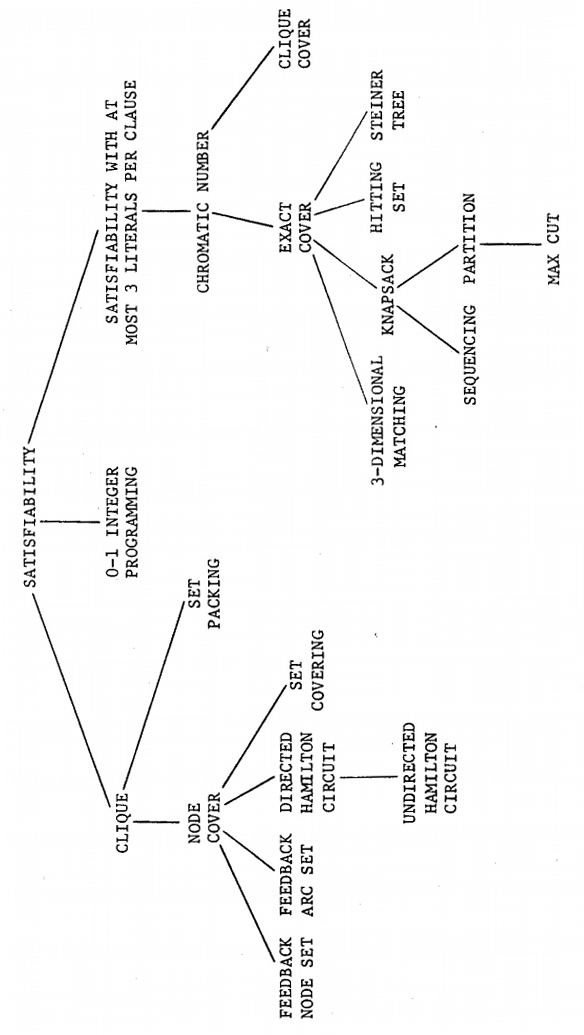
\includegraphics[width=12cm]{complete_problems.png}
        \caption{完全问题}
    \end{figure*}

    很明显,这些问题(更准确的说是他们在$\Sigma^*$中的编码)都属于$\mathcal{NP}$。我接下来将构造一系列的规约,证明$SAT$问题是可以规约到上面列出的每一个问题。图-1显示了这一系列的规约的过程。图中每一条线都代表一个从位置靠上的问题到位置靠下的问题的规约。

    为了展示从集合$T\subset D$到集合$T'\subset D'$的规约。我们需要找到满足引理2的函数$F:D\rightarrow D'$。对于接下来我们给出的每个规约,读者可以很容的验证他们满足那些条件。
    \begin{itemize}
    \item 可满足性问题(SAT)$\propto$ 0-1整数规划
        \begin{equation}\nonumber % Remove numbering (before each equation)
        \begin{aligned}
            &c_{ij}=\left\{
            \begin{matrix}
              1 & \text{如果}x_j\in C_i \\
              -1 & \text{如果}\bar{x_j}\in C_i \\
              0 & \text{其它}
            \end{matrix}
            \right.
            \qquad
            \begin{matrix}
              i=1,2,\cdots,p\\
              j=1,2,\cdots,n
            \end{matrix}
            \\
            &b_i=1-(C_i\text{中取补的变量个数})
        \end{aligned}
        \end{equation}
        
    \item 可满足性问题 $\propto$ 分团问题
        \begin{equation}\nonumber % Remove numbering (before each equation)
        \begin{aligned}
        & N = \{<\sigma,i>|\sigma\text{是}C_i\text{中出现的文字(Literal)}\} \\
        & A = \{\{<\sigma,i>,<\delta,j>\}|i\neq j\text{且}\sigma\neq\bar{\delta}\} \\
        & k = p\text{,分团数}
        \end{aligned}
        \end{equation}

    \item 分团问题 $\propto$ SET PACKING
        假设$N=\{1,2,\cdots,n\}$。集合$S_1,S_2,\cdots,S_n$中的元素是那些不在$A$中的节点二元集$\{i,j\}$。
        \begin{equation}\nonumber % Remove numbering (before each equation)
        \begin{aligned}
        & S_i=\{\{i,j\}|\{i,j\}\notin A\},\ i=1,2,\cdots,n\\
        & \ell=k
        \end{aligned}
        \end{equation}

    \item 分团问题 $\propto$ 顶点覆盖
        \begin{equation}\nonumber % Remove numbering (before each equation)
        \begin{aligned}
        & G' \text{是}G\text{补图}\\
        & \ell=|N|-k
        \end{aligned}
        \end{equation}

    \item 顶点覆盖 $\propto$ 集合覆盖\\
    
        假设$N'=\{1,2,\cdots,n\}$。则(集合覆盖问题中的集合的)元素为$G'$中的边。$S_j$是节点$j$的临边组成的集合。最后,$k=\ell$。

    \item 顶点覆盖 $\propto$ 反馈顶点集
        \begin{equation}\nonumber % Remove numbering (before each equation)
        \begin{aligned}
        & V=N'
        & E=\{<u,v>|\{u,v\}\in A'\}
        & k=\ell
        \end{aligned}
        \end{equation}

    \item 顶点覆盖 $\propto$ 反馈边集
        \begin{equation}\nonumber % Remove numbering (before each equation)
        \begin{aligned}
        V=&N'\times\{0,1\}\\
        E=&\{<<u,0>,<u,1>>|u\in N'\}\\
          &\cup\{<<u,1>,<v,0>>|\{u,v\}\in A'\}\\
        k=&\ell
        \end{aligned}
        \end{equation}

    \item 顶点覆盖 $\propto$ 有向汉密尔顿回路\\
        不失一般性的,我们假设$A'=Z_m$。
        \begin{equation}\nonumber % Remove numbering (before each equation)
        \begin{aligned}
        V=  &\{a_1,a_2,\cdots,a_\ell\}\\
            &\cup\{<u,i,\alpha>|u\in N'\text{与}i\in A'\text{连接,且}\alpha\in \{0,1\}\}\\
        E=  &\{<<u,i,0>,<u,i,1>>|<u,i,0>\in V\}\\
            &\cup\{<<u,i,\alpha>,<v,i,\alpha>>|i\in A',\\
                &\hphantom{\cup\{<<u,i,\alpha>,}\text{u和v与i连接,且}\alpha\in \{0,1\}\}\\
            &\cup\{<<u,i,1>,<u,j,0>>|u\text{和}i,j\text{连接},\\
                &\hphantom{\cup\{<<u,i,}\text{且不存在h,同时满足}i<h<j\text{和u与h相邻}\}\\
            &\cup\{<<u,i,1>,a_f>|1\leq f\leq\ell, \\
                &\hphantom{\cup\{<<u,i,}\text{且不存在}h > i,\text{使得u与h连接}\}\\
            &\cup\{<a_f,<u,i,0>>|1\leq f\leq\ell, \\
                &\hphantom{\cup\{<<u,i,}\text{且不存在}h < i,\text{使得u与h连接}\}\\
        \end{aligned}
        \end{equation}

    \item 有向汉密尔顿回路 $\propto$ 无向汉密尔顿回路
        \begin{equation}\nonumber % Remove numbering (before each equation)
        \begin{aligned}
        N=  &V\times{0,1,2}\\
        A=  &\{\{<u,0>,<u,1>\},\{<u,1>,<u,2>\}|u\in V\}\\
            &\cup\{\{<u,2>,<v,0>\}|<u,v>\in E\}
        \end{aligned}
        \end{equation}

    \item 可满足性问题 $\propto$ 3-可满足性问题\\
        把每个满足$\sigma_i$是文字且$m>3$的语句$\sigma_1\cup\sigma_2\cup\cdots\cup\sigma_m$替换为:
        $$(\sigma_1\cup\sigma_2\cup u_1) (\sigma3\cup\cdots\cup\sigma_m\cup\bar{u}_1)
        (\bar{\sigma}_3\cup u_1) \cdots(\bar{\sigma}_m\cup u_1)$$
        其中$u_1$是一个新的变量。重复这个变换直到没有语句有多于三个的文字。

    \item 3-可满足性问题 $\propto$ 色数\\
        不失一般性的,我们假设$m>4$。
        \begin{equation}\nonumber % Remove numbering (before each equation)
        \begin{aligned}
        N=  &\{u_1,u_2,\cdots,u_m\}\cup
                \{\bar{u}_1,\bar{u}_2,\cdots,\bar{u}_m\}\cup\\
            &\{v_1,v_2,\cdots,v_m\}\cup
                \{D_1,D_2,\cdots,D_r\}\\
        A=  &\{\{u_i,\bar{u}_i\}|i=1,2,\cdots,n\}\cup\{\{v_i,v_j\}|i\neq j\}\cup\\
            &\{\{v_i,x_j\}|i\neq j\}\cup\{\{v_i,\bar{x}_j\}|i\neq j\}\cup\\
            &\{\{u_i,D_f\}|u_i\notin D_f\}\cup\{\{\bar{u}_i,D_f\}|\bar{u}_i\notin D_f\}\\
        k=&r+1
        \end{aligned}
        \end{equation}

    \item 色数 $\propto$ 分团覆盖
        \begin{equation}\nonumber % Remove numbering (before each equation)
        \begin{aligned}
        & G'\text{是}G\text{的补图}\\
        & \ell=k
        \end{aligned}
        \end{equation}

    \item 色数 $\propto$ 精确覆盖\\
        精确覆盖问题中的集合为
        $$N\cup A\cup\{<u,e,f>|u\text{与}e\text{连接且}1\leq f \leq k\}$$
        族$\{S_j\}$构造如下:\\
        对满足$1\leq f \leq k$的所有f,和所有$u\in N$,\\
        $$\{u\}\cup\{<u,e,f>|e\text{与}u\text{连接}\}\in\{S_j\}$$\\
        对于所有$e\in A$和所有满足$1\leq f_1 \leq k,1\leq f_2 \leq k,f_1\neq f_2$的$f_1,f_2$
        \begin{equation}\nonumber % Remove numbering (before each equation)
        \begin{aligned}
        &\{e\}\cup\{<u,e,f>,f\neq f_1\}\\
        &\hphantom{\{e\}\cup\{<u,}\cup\{<v,e,g>,g\neq f_2\} \in\{S_j\}\\
        &\text{其中}u\text{和}v\text{是和}e\text{连接的两个节点。}
        \end{aligned}
        \end{equation}
        其余集合都不属于$\{S_j\}$。

    \item 精确覆盖 $\propto$ 碰集\\
        碰集有集合$U_i$和元素$s_j$,使得$s_j\in U_i\Leftrightarrow u_i\in S_j$。

    \item 精确覆盖 $\propto$ 斯坦纳树
        \begin{equation}\nonumber % Remove numbering (before each equation)
        \begin{aligned}
        &N=\{n_o\}\cup\{S_j\}\cup\{u_i\}\\
        &R=\{n_o\}\cup\{u_i\}\\
        &A=\{\{n_o,S_j\}\}\cup\{\{S_j,u_i\}|u_i\in S_j\}\\
        &w(\{n_o,S_j\})=|S_j|\\
        &w(\{S_j,u_i\})=0\\
        &k=|\{u_i\}|
        \end{aligned}
        \end{equation}

    \item 精确覆盖 $\propto$ 3维匹配\\
        不失一般性的,我们假设$|S_j|>2$对于所有$j$。令$T=\{<i,j>|u_i\in S_j\}$。令$\alpha$是任意一个从$\{u_i\}$到$T$的一对一函数。令$\pi:T\rightarrow T$是一个置换,使得对每一个固定的j,$\{<i,j>|u_i\in S_j\}$是$\pi$的周期。
        \begin{equation}\nonumber % Remove numbering (before each equation)
        \begin{aligned}
        U=&\{<\alpha(u_i),<i,j>,<i,j>>|<i,j>\in T\}\\
          &\cup\{<\beta,\sigma,\pi(\sigma)>|\text{对所有}i,\beta\neq \alpha(u_i)\}
        \end{aligned}
        \end{equation}

    \item 精确覆盖 $\propto$ 背包问题\\
        令$d=|\{S_j\}|+1$。令$\epsilon_{ji}=
        \left\{\begin{matrix}
            1 & \text{如果}u_i\in S_j \\
            0 & \text{如果}u_i\notin S_j 
        \end{matrix}\right.$ 令$r=|\{S_j\}|$。
        
        \begin{equation}\nonumber % Remove numbering (before each equation)
        \begin{aligned}
        &a_j=\sum\epsilon_{ji}d^{i-1}\\
        &b=\frac{d^t-1}{d-1}
        \end{aligned}
        \end{equation}

    \item 背包问题 $\propto$ 工作排序
        $$p=r, T_i=P_i=a_i, D_i=b.$$

    \item 背包问题 $\propto$ 集合划分
        \begin{equation}\nonumber % Remove numbering (before each equation)
        \begin{aligned}
        &s=r+2\\
        &c_i=a_i,i=1,2,\cdots,r\\
        &c_{r+1}=b+1\\
        &c_{r+2}=(\sum_{i=1}^{r}a_i)+1-b\\
        \end{aligned}
        \end{equation}

    \item 集合划分 $\propto$ 最大割
        \begin{equation}\nonumber % Remove numbering (before each equation)
        \begin{aligned}
        &N=\{1,2,\cdots,s\}\\
        &A=\{\{i,j\}|i\in N,j\in N,i\notin j\}\\
        &w(\{i,j\})=c_i\cdot c_j\\
        &W=\lceil \frac14\sum c_i^2\rceil
        \end{aligned}
        \end{equation}

    \end{itemize}
% \section{理论分析}
%     \subsection{稀疏矩阵}
%     稀疏矩阵采用二维链表的方式进行储存,可以高效的进行矩阵乘法,加快Gauss-Seidel方法和Conjugate Gradient方法的运算速度。二维链表结构如\figurename\ref{2DimensionLinkedList}所示。每个非零元素都储存为一个节点。节点中除了包含该节点的值、行号、列号以外,还存有两个指针,分别指向同一行的下一个节点和同一列的下一个节点。而所有的行的头指针和列的头指针则存在两个数组中。对于一个含有$m$个元素的规模为$n\times n$的稀疏矩阵,所需存储空间为$O(m+n)$。
%     % \begin{figure}
%     % \center
%     % \includegraphics[width=9cm]{pictures/2DimensionLinkedList.png}
%     % \caption{稀疏矩阵储存结构}\label{2DimensionLinkedList}
%     % \end{figure}
%         \subsubsection{\tt at(row, col)}
%         这个函数内部实现方式是遍历第row行的节点,找到列号与col相等的节点。之后将该节点的值返回。如果没找到,则返回0。时间复杂度取决于该行有多少个元素。如果$m$个元素在$n$行分布均匀的话,则平均时间复杂度为$O(m/n)$。

%         \subsubsection{\tt insert(val, row, col)}
%         首先要判断第row行、第col列的节点是否在链表中。如果在,且val不为0,则直接更改节点值为val。如果在,但是val为0,则删去这个节点。如果节点不在链表中,且val值不为0,则创建这个节点,插入链表中。因为要使每行的列号和每列的行号保持递增的顺序,所以插入时需要逐个遍历所在行和所在列。时间复杂度取决于要插入的行和列的节点个数。如果$m$个元素均匀分布在$n$行和$n$列,则时间复杂度为$O(m/n)$

%         \subsubsection{\tt initializeFromVector(rows,cols,vals)}
%         这个实现方式不同于CRC和CRS。对于这种结构,如果矩阵稀疏的话,多次连续插入,直接调用insert即可。再优化的话,也只有常数级别的时间减少。

%         \subsubsection{\tt 矩阵乘法}
%         对$r\times s$稀疏矩阵$A$和$s\times t$的稀疏矩阵$B$进行乘法运算,如果$A$有$n$个非零元素,$B$有$m$个非零元素,则时间复杂度为$O(nt+mr)$。因为$n\leq rs$且$m \leq st$,所以这个乘法要快于直接按乘法定义进行计算的$O(rst)$。
%     \subsection{Gauss-Seidel Method}
%     求解线性方程组$AX=b$。将$A$分解为下三角矩阵$L_*$和严格上三角矩阵$U$,之后进行迭代:$$L_*x^{(k+1)}=b-Ux^{(k)}$$迭代过程也可写作$$x_i^{(k+1)}=\frac{1}{a_{ii}}\left(b_i-\sum_{j<i}a_{ij}x_j^{(k+1)}-\sum_{j>i}a_{ij}x_j^{(k)}\right)$$这就是Gauss-Seidel Method。如果A是对称正定阵,或者严格或不可约对角占优,则这个迭代一定收敛。实现上与Jacobi Method相似,不过每次计算出新的X中的元素就立即更新X,让更新的元素立刻参与下一个元素的计算。相比Jacobi Method收敛速度快很多。

%     \subsection{Conjugate Gradient Method}
%     Conjugate Gradient是一种迭代求解线性方程组的方法。对于有唯一解$X_*$的线性方程组$AX=b$,如果$A$是实对称正定阵,则函数
%     $$f(X)=\frac{1}{2}X^TAX-X^Tb$$
%     当且仅当$X=X_*$时,取到最小值。所以求解$AX=b$的问题转变为
%     $$\min f(X)$$
%     常用的求函数最小值的方法有梯度下降法。但是梯度下降法实际上是一种贪心算法,收敛速度慢。共轭梯度法则是在每次迭代时,都选取与当前向量$X^{(k)}$共轭的方向进行优化。对于$n\times n$的矩阵A,最多迭代$n$次即可获得精确解,收敛速度快于梯度下降法。具体算法见下页$Algorithm$ \ref{Conjugate Gradient Algorithm}。
%     \begin{algorithm}
%       \caption{Conjugate Gradient Method}
%       \label{Conjugate Gradient Algorithm}
%       \begin{algorithmic}[1]
%         \STATE $r_0:=b-AX_0$
%         \STATE $p_0:=r_0$
%         \STATE $k:=0$
%         \LOOP
%             \STATE $\alpha_k:=\frac{r_k^Tr_k}{p_k^TAp_k}$
%             \STATE $x_{k+1}:=x_k+\alpha_kp_k$
%             \STATE $r_{k+1}:=r_k-\alpha_kAp_k$
%             \IF{$r_{k+1}$is sufficiently small}
%                 \STATE Exit Loop
%             \ENDIF
%             \STATE $\beta_k:=\frac{r_{k+1}^Tr_{k+1}}{r_k^Tr_k}$
%             \STATE $p_{k+1}:=r_{k+1}+\beta_kp_k$
%             \STATE $k:=k+1$
%         \ENDLOOP
%         \STATE $x_{k+1}$is the result
%         % \FORALL {$v \in V(G)$}
%             % \STATE $l(v) \leftarrow \infty$
%         % \ENDFOR
%       \end{algorithmic}
%     \end{algorithm}



% \section{实现细节}
%     对于稀疏矩阵全都使用自己实现的模版{\tt SparseMatrix<DataType>}来存储。对于列向量全部使用STL标准库中的{\tt std::vector<DataType>来储存}。Gauss-Seidel Method和Conjugate Gridient Method实现为两个函数模版。所有的模版都在{\tt SparseMatrix.h}中。
%     \subsection{稀疏矩阵\tt SparseMatrix<DataType>}
%     对于稀疏矩阵,我实现了模版{\tt SparseMatrix<DataType>}。模版是比较适合来实现矩阵这种通用的数据类型的。以后可以很方便的指定是整型矩阵或浮点型矩阵,甚至是虚数矩阵。主要成员函数如下:
%     \begin{itemize}
%     \item {\tt SparseMatrix(int rows, int cols); $\backslash\backslash$构造函数}
%     \item {\tt \verb1~1SparseMatrix(); $\backslash\backslash$析构函数}
%     \item {\tt DataType at(unsigned int row, unsigned int col); $\backslash\backslash$获得指定位置的值}
%     \item {\tt void insert(DataType val, unsigned int row, unsigned int col); $\backslash\backslash$插入一个元素}
%     \item {\tt void initializeFromVector(std::vector<int>\& rows, \newline
%         \hphantom{void initializeFromVector(}std::vector<int>\& cols, \newline
%         \hphantom{void initializeFromVector(}std::vector<DataType>\& vals) $\backslash\backslash$ 从向量初始化}
%     \end{itemize}
%     非成员函数如下:
%     \begin{itemize}
%     \item {\tt void mul(const SparseMatrix<DataType>\& left, \newline
%         \hphantom{void mul(}const std::vector<DataType>\& right, \newline
%         \hphantom{void mul(}std::vector<DataType>\& result); $\backslash\backslash$矩阵$\times$列向量}
%     \item {\tt void mul(const SparseMatrix<DataType>\& left, \newline
%         \hphantom{void mul(} const SparseMatrix<DataType>\& right, \newline
%         \hphantom{void mul(}SparseMatrix<DataType>\& result); $\backslash\backslash$矩阵$\times$矩阵}
%     \item {\tt std::ostream\& operator<< (std::ostream\& os, \newline
%         \hphantom{std::ostream\& operator<< (}SparseMatrix<DataType>\& mat)$\backslash\backslash$输出矩阵为可读字符串,方便调试}
%     \end{itemize}

%     \subsection{Gauss-Seidel Method}
%     {\tt void gaussSeidel(SparseMatrix<DataType>\& A, \newline
%         \hphantom{void gaussSeidel(}std::vector<DataType>\& b, \newline
%         \hphantom{void gaussSeidel(}std::vector<DataType>\& X, $\backslash\backslash$求解结果\newline
%         \hphantom{void gaussSeidel(}DataType accuracy $\backslash\backslash$精度\newline
%         \hphantom{void gaussSeidel(});}\\
%     函数进行了矩阵大小的检查,保证$A$的行数和$b$的行数是一样的,如果不一样则退出程序。但是并不会检查$A$是否满足收敛条件。需要使用者自己保证收敛。

%     \subsection{Conjugate Gridient Method}
%     {\tt void conjugateGridient(SparseMatrix<DataType>\& A, \newline
%         \hphantom{void conjugateGridient(}std::vector<DataType>\& b, \newline
%         \hphantom{void conjugateGridient(}std::vector<DataType>\& X, $\backslash\backslash$求解结果\newline
%         \hphantom{void conjugateGridient(}DataType accuracy $\backslash\backslash$精度\newline
%         \hphantom{void conjugateGridient(});}\\
%     函数进行了矩阵大小的检查,保证$A$的行数和$b$的行数是一样的,如果不一样则退出程序。但是并不会检查$A$是否是实对称正定阵。需要使用者自己保证$A$是实对称正定阵。

% \subsection{实验结果}
%     {\tt main.cpp}中的{\tt main}函数是一个简单的测试程序。首先使用initializeFromVector生成一个如下的$100,000\times100,000$的实对称正定阵稀疏矩阵$A$。再生成如下一个列向量$b$。
%     $$\begin{bmatrix}
%         3&1&      &      &\\
%         1&3&1     &      &\\
%          &1&\ddots&\ddots&\\
%          & &\ddots&3     &1\\
%          & &      &1     &3\\
%     \end{bmatrix}
%     X=
%     \begin{bmatrix}
%         0 \\
%         1 \\
%         \vdots \\
%         \vdots \\
%         100000 \\
%     \end{bmatrix}
%     $$
%     设置精度为$10^{-9}$,使用两种方法求解线性方程组$AX=b$。Gauss-Seidel Method用时3.237s。Conjugate Gridient Method用时8.823s。而且两种方法计算结果十分接近,说明求解结果正确。运行中打印信息如下,截图见\figurename\ref{run}。
%     \begin{verbatim}Generating A and b.
% Solving AX=b.
% A is of size 100000*100000.
% Error is required to be smaller than 1e-009.
% Using Gauss-Seidel Method...
% Gauss-Seidel method took 3.237 seconds.
% Using Conjugate Gridient Method...
% Conjugate Gridient method took 8.823 seconds.
% Difference of the two solutions is less than 4.65661e-010\end{verbatim}
%     % \begin{figure}
%     % \center
%     % \includegraphics[]{pictures/run.png}
%     % \caption{运行结果}\label{run}
%     % \end{figure}

%     除此之外还曾构造过多个测试样例进行测试,以保证程序正确性。
\end{CJK}
\end{document} 